\section{Wstęp}
\subsection{Wprowadzenie}

Celem projektu jest opracowanie programu umożliwiającego przeprowadzenie symulacji wybranych rozwiązań warstwy fizycznej Ethernet.
Przyjęty, wraz z promotorem, zakres prac zakłada realizację następujących elementów:
\begin{itemize}
    \item symulację sygnału w skrętce z możliwością modyfikacji parametrów wejściowych oraz kanału
    \item symulację wybranch modulacji PAM
    \item symulację kodowania korekcyjnego Reeda-Solomona
\end{itemize}

Ponad to, w ramach pracy inżynierskiej, dyplomanci przygotują scenariusz zajęć laboratoryjnych wykorzystujących opracowany symulator, jak
również przeprowadzą te zajęcia z grupą studentów. Scenariusz zawrze takie elementy jak wstęp teoretyczny do omawianych zagadnień,
zadania na wejściówkę, zadania do realizacji na laboratoriach oraz opracowanie wymienionych zadań.

Podczas przygotowywania dyplomu, autorzy zapoznają się ze standardem IEEE 802.3, specyfiką oraz problemami występującymi w warstwie fizycznej
w sieciach Ethernet. Dzięki realizacji tych zadań, dyplomanci poszerzą swoją wiedzę w wymienionych obszarach oraz podzielą się wynikami
swojej pracy ze studentami.

\section{Środowisko programistyczne}
\subsection{Język programowania}

Do stworzenia symulatora wybrano język programowania Python z uwagi na kilka istotnych powodów. Przede wszystkim, czytelność składni stanowi ogromne ułatwienie podczas wspólnego tworzenia oprogramowania, a prostota pozwala skupić się na istocie problemu, nie tracąc czasu na pokonywanie trudności języka.

Dodatkowo, wybór Pythona jest motywowany chęcią rozwijania naszych umiejętności w tym środowisku, zarówno na poziomie indywidualnym, jak i zawodowym. Python cieszy się dużą popularnością jako uniwersalny język programowania, używany w różnych dziedzinach, takich jak analiza danych, sztuczna inteligencja czy aplikacje webowe. Posiadanie umiejętności programowania w Pythonie otwiera drzwi do szerszych możliwości zawodowych i dostępu do różnorodnych ciekawych projektów.

Jednym z najważniejszych argumentów przemawiających za wyborem Pythona jest jego ogromna popularność. Związana z tym społeczność programistyczna tworzy rozbudowany ekosystem, oferujący dostęp do wielu gotowych rozwiązań, bibliotek i frameworków. W kontekście tworzenia symulatora, istnieje wiele bibliotek w Pythonie, które mogą okazać się niezwykle przydatne. Na przykład, biblioteki umożliwiające tworzenie interfejsów graficznych ułatwią korzystanie z symulatora, biblioteki do analizy i przetwarzania sygnałów pomogą modelować różne aspekty transmisji, a biblioteki do wizualizacji pozwolą na przedstawienie wyników w przystępny sposób.

Inną cechą, która wyróżnia ten język programowania, jest jego przenośność. To ma dla nas duże znaczenie przy tworzeniu symulatora, który musi działać w warunkach laboratoryjnych, a więc na dowolnym popularniejszym systemie operacyjnym oraz charakteryzować się łatwością instalacji. Te wymagania Python w naszej ocenie spełnia.

\subsection{Narzędzia, biblioteki i moduły}
Jednym z celów postawionych przez promotora jest wykorzystanie gotowych rozwiązań podczas pracy nad symulatorem. W tym rozdziale zostaną przedstawione biblioteki i moduły języka Python oraz inne narzędzia, które mogą zostać wykorzystane w programie.

Python oferuje wiele bibliotek, które mogą okazać się kluczowe: od interfejsu graficznego po gotowe narzędzia do symulacji. Oto przegląd kilku z nich, na które brano pod uwagę przy projektowaniu rozwiązania:

\begin{enumerate}
    \item PyQt będzie biblioteką wykorzystywaną do stworzenia interfejsu graficznego użytkownika (GUI) dla symulatora. PyQt zapewnia szeroki zakres narzędzi do tworzenia rozbudowanych i przyjaznych użytkownikowi interfejsów, co jest szczególnie ważne w symulatorze dydaktycznym, gdzie interfejs musi być intuicyjny i nie stanowić niepotrzebnego wyzwania lub problemu dla biorących udział studentów
    \item NumPy jest najpopularniejszą biblioteką Python implementującą algorytmy matematyczne. Między innymi oferuje generatory liczb pseudolosowych o różnych rozkładach, co jest wymagane do prawidłowego generowania ramek ethernetowych i błędów
    \item  Matplotlib to popularna biblioteka do tworzenia wykresów. Może okazać się przydatna przy tworzeniu wykresów sygnałów
\end{enumerate}


Istnieją również inne popularne narzędzia, które mogą być użyteczne do symulacji rozwiązań warstwy fizycznej sieci Ethernet:
\begin{enumerate}
    \item SPICE (Simulation Program with Integrated Circuit Emphasis) jest powszechnie stosowanym narzędziem do symulacji obwodów elektronicznych. Jest to rozbudowany program, który umożliwia modelowanie i analizę zachowania obwodów złożonych, takich jak układy analogowe, cyfrowe czy mikroelektroniczne. W celu korzystania z tego narzędzia w środowisku Python dostępna jest biblioteka PySpice, będąca interfejsem umożliwiającym korzystanie ze SPICE,
    \item MATLAB to znane i powszechnie używane narzędzie do obliczeń numerycznych, analizy danych i modelowania systemów. Posiada szeroki zakres narzędzi i funkcji przeznaczonych do tworzenia modeli matematycznych, symulacji dynamicznych itp.,
    \item Scapy umożliwia tworzenie i przetwarzanie różnego rodzaju pakietów sieciowych, w tym ramek Ethernet, co jest kluczową funkcjonalnością symulatora.
\end{enumerate}

\section{Symulator}
\subsection{Interfejs użytkownika}
Interfejs użytkownika został wykonany przy użyciu PyQt5 oraz Qt Designer. Qt Designer to graficzne narzędzie do projektowania interfejsów użytkownika w ramach frameworka Qt. Umożliwia łatwe tworzenie i dostosowywanie wyglądu aplikacji oraz następne jego wygenerowanie jako kodu w języku Python lub C++.

Interfejs składa się z kilku zakładek stworzonych, które umożliwiają przełączanie między częściami aplikacji bez utraty wyników dotychczasowej pracy. Każda zakładka przeznaczona jest do innego zadania laboratoryjnego i zawiera symulacje innych rozwiązań ethernetowych. 

\begin{figure}[ht]
    \centering
    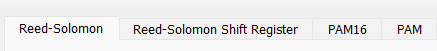
\includegraphics{images/zakladki.png}
    \caption{Zakładki symulatora}
    \label{fig:zakladki_image}
\end{figure}

Wykresy są tworzone przy pomocy biblioteki Matplotlib. Została dodatkowo stworzona klasa, która zawiera stworzone wykresy i może być użyta jako element graficznego interfejsu użytkownika, a więc dodana do niego.

\subsection{Symulacje wybranych rozwiązań}
Aplikacja umożliwa symulowanie wybranych rozwiązań fizycznej warstwy sieci Ethernet. W każdym przypadku użytkownik ma swobodę podawania własnych parametrów wejściowych, zmieniania ich, co ma na celu ułatwienie zrozumienia działania tych rozwiązań.

\subsubsection{Kodowanie korekcyjne Reeda-Solomona}
Kodowanie korekcyjne Reed-Solomona to metoda kodowania korekcyjnego, mająca na celu wykrywanie i naprawianie błędów w przesyłanych danych. Stworzona została w 1960 roku przez dwóch amerykańskich matematyków: Irving S. Reed i Gustave Solomon. Od tego czasu znalazła szerokie zastosowanie w dziedzinie komunikacji, kodowaniu i obsłudze dysków.

Główną ideą kodowania korekcyjnego Reed-Solomona jest dodawanie nadmiarowych danych do przesyłanych informacji, dzięki czemu w przypadku wystąpienia błędów, możliwe jest ich wykrycie i skorygowanie. Algorytm opiera się na algebraicznych właściwościach ciał skończonych, co umożliwia efektywne wykonywanie operacji matematycznych potrzebnych do kodowania i dekodowania.

W symulatorze kodowanie i dekodowanie wykorzytuje metody klasy ReedSolomon udostępnionej w bibliotece galois. Jest ona rozszerzeniem, dodającym operacje na ciałach skończonych, innej popularnej biblioteki języka Python - NumPy. Jej nazwa pochodzi od nazwiska francuskiego matematyka Évariste Galois, który zasłynął badaniami ciał skończonych, które nazywane są również ciałami Galois.

\begin{figure}[ht]
    \centering
    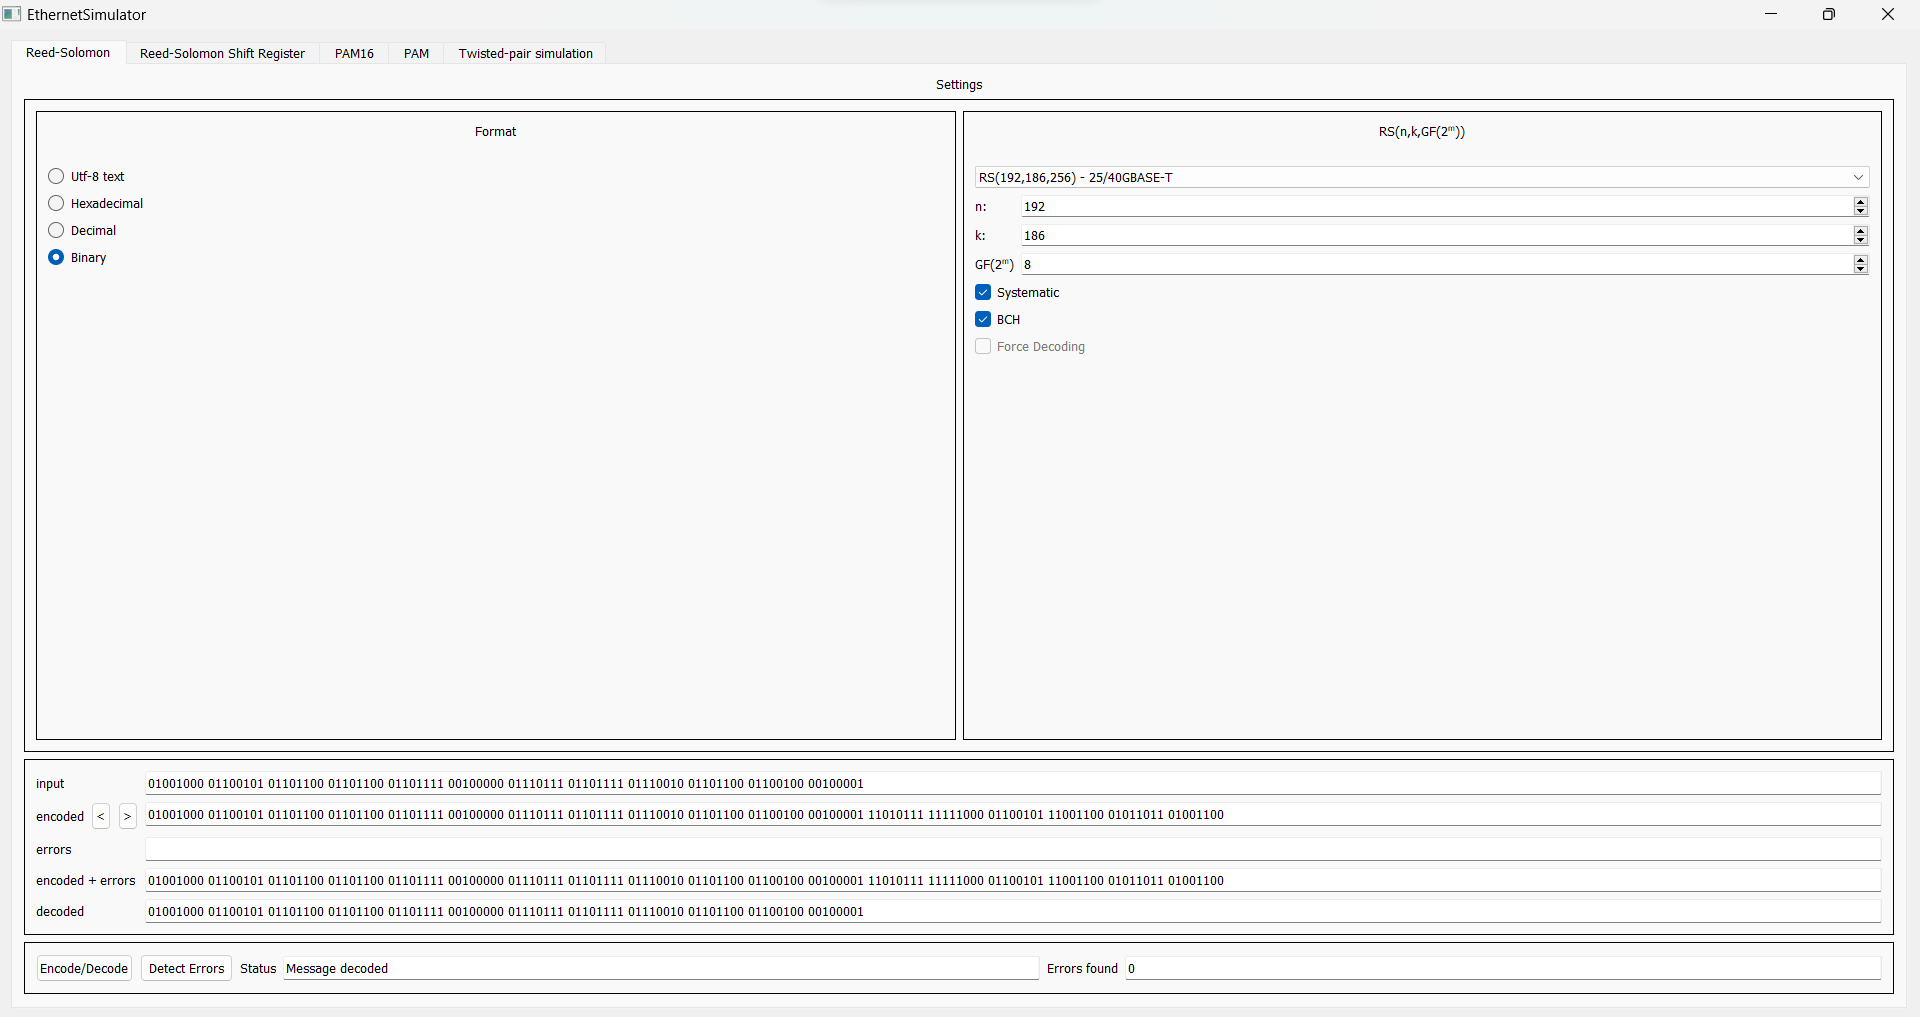
\includegraphics[width=\textwidth]{images/rs.png}
    \caption{Zakładka z kodowaniem Reeda-Solomona}
    \label{fig:rs_image}
\end{figure}

\subsubsection{Symulacja przesyłu sygnału}
Symulator umożliwia symulację przesyłu danych przez pojedynczą lub 4-parową skrętkę, w której można śledzić zmiany napięć. W tym przypadku wykorzystana została biblioteka PySpice. Dzięki niej można nadać wykorzystywanemu przewodowi pożądane parametry, między innymi: opór, długość i indukcyjność.

Użytkownik ma możliwość podawania tych parametrów w przewijalnym oknie, gdzie może dodawać również kolejne przewodniki. Patrz Table~\ref{tab:parametry}.

\begin{table}[ht]
    \centering
    \begin{tabular}{|c|c|c|c|}
        \hline
        \textbf{Parametr} & \textbf{Od} & \textbf{Do} & \textbf{Domyślnie} \\
        \hline
        Voltage offset & 0 & 10 & 0 \\
        Output impedance & 0 & 200 & 100 \\
        Length & 1 & 100 & 2 \\
        Resistence & 0 & 100 & 0.19 \\
        Inductance & 0 & 1000 & 525 \\
        Capacitance & 0 & 100 & 52 \\
        \hline
    \end{tabular}
    \caption{Parametry symulacji}
    \label{tab:parametry}
\end{table}

Symulacja wykonywana jest w osobnym wątku. Dodatkowo możliwa jest jednoczesna symulacja wielu przewodów o różnych parametrach, które następnie przedstawiane są na jednym wykresie. Opcjonalnie można ukrywać lub pokazywać wybrane symulacji zaznaczając odpowiednie pola przy listach parametrów odpowiednich przewodów.

\begin{figure}[ht]
    \centering
    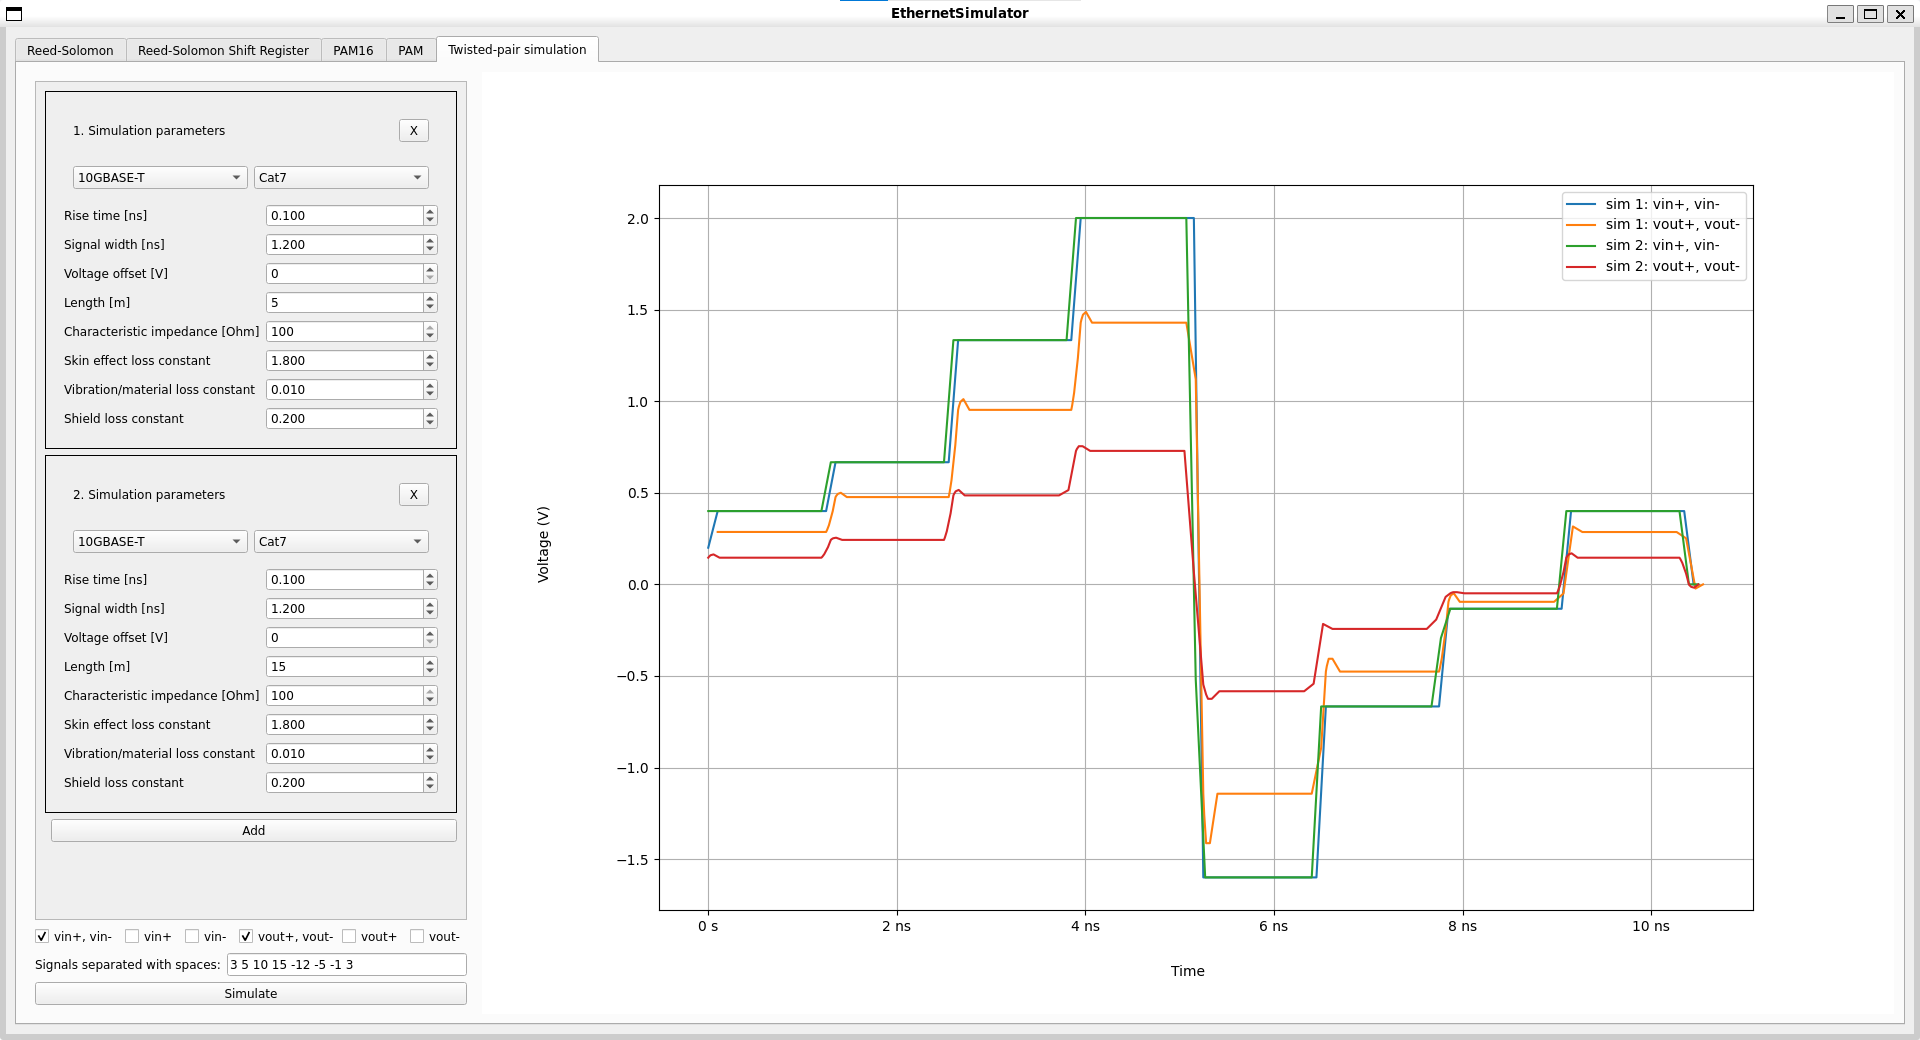
\includegraphics[width=\textwidth]{images/sim.png}
    \caption{Zakładka z symulacją}
    \label{fig:sim_png}
\end{figure}